\documentclass{standalone}
    \usepackage{xeCJK}
    \usepackage{tikz}
    \usetikzlibrary{shapes.geometric, arrows.meta, arrows,positioning}
    
  \begin{document}
  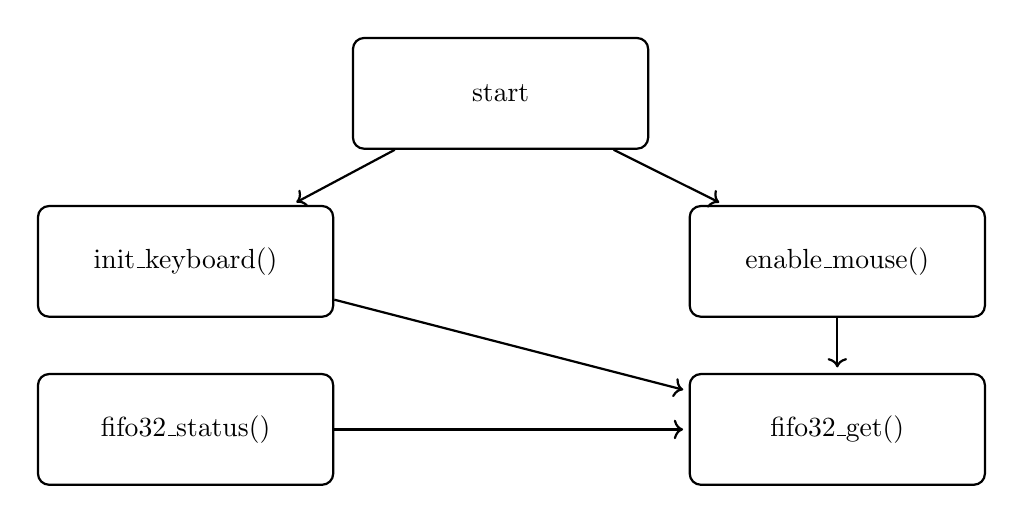
\begin{tikzpicture}
    [auto,
    block/.style={rectangle, draw=black, thick,
    text width=10em,align=center, rounded corners,
    minimum height=4em},
    line/.style={draw, thick, shorten >=2pt, ->}]
  
    \matrix [column sep=5mm,row sep=7mm]
    {
        \node [block] (start) {start}; \\

        \node [block] (init_kbd)[xshift=-4cm]{init\_keyboard()}; & 
        \node [block] (eab_ms)[xshift=1cm]{enable\_mouse()}; \\

        \node [block] (fifo_status) [xshift=-4cm]{fifo32\_status()}; & 
        \node [block] (fifo32_get) [xshift=1cm]{fifo32\_get()}; \\
    };
    \begin{scope}[every path/.style=line]
        \path (start) -- (init_kbd);
        \path (start) -- (eab_ms);
        \path (fifo_status) -- (fifo32_get);
        \path (init_kbd) -- (fifo32_get);
        \path (eab_ms) -- (fifo32_get);
    \end{scope}
    \end{tikzpicture}
\end{document}
  
  %%% Local Variables:
  %%% mode: latex
  %%% TeX-master: t
  %%% End:
  